\newpage
\section*{Referencias}
\textbf{Básico: } Prueba de la ronda Final de OMAPA 2012, Nivel 1, Grados 6 y 7. \\
\textbf{Medio: } Prueba de la ronda Final de OMAPA 2012, Nivel 2, Grados 8 y 9. \\
\textbf{Avanzado: } Prueba de la ronda Final de OMAPA 2012, Nivel 3, Grados 10 y 11

%------------------------------------------------------------------------------------------------------------   
%----------------------------------                        BASICO                       ---------------------------------- 
%------------------------------------------------------------------------------------------------------------ 

\newpage
\section{Nivel Básico}\label{BASICO_2020_23_mayo}

\begin{center}
	\fbox{\fbox{\parbox{6in}{\centering
				\textbf{Tiempo mínimo: } 2 horas y 30 minutos.\\
				\textbf{Tiempo máximo: } 4 horas.\\	
				\textbf{Procedimientos: }Cada problema debe estar resuelto por escrito, en forma detallada, todos los pasos seguidos para su resolución deben estar bien explicados. Se le brindarán unas hojas grapadas, en la \textit{parte de enfrente} de cada hoja debe estar la solución de los problemas, la \textit{parte posterior} no se leerá pero las operaciones y cálculos deben hacerlos allí. \\
				\textbf{Puntaje: }Cada problema vale 50 puntos, son 5, para un total de 250 puntos.
				}}}
\end{center}


\begin{figure}[H]
	\centering
	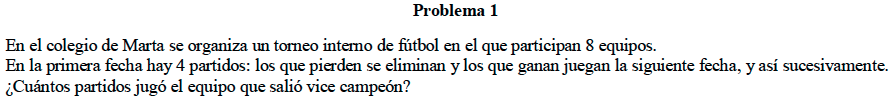
\includegraphics[width=\linewidth]{2020_05_23/imgs/OMAPA_2012_r5_B_1}
	%\caption{}
	\label{OMAPA_2012_r5_B_1}
\end{figure}

\begin{figure}[H]
	\centering
	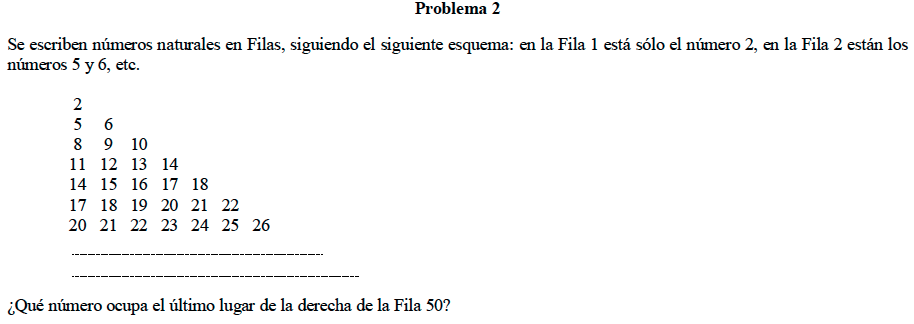
\includegraphics[width=\linewidth]{2020_05_23/imgs/OMAPA_2012_r5_B_2}
	%\caption{}
	\label{OMAPA_2012_r5_B_2}
\end{figure}

\begin{figure}[H]
	\centering
	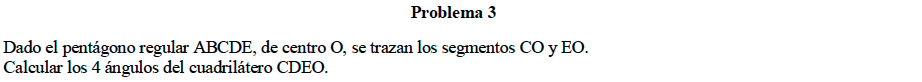
\includegraphics[width=\linewidth]{2020_05_23/imgs/OMAPA_2012_r5_B_3}
	%\caption{}
	\label{OMAPA_2012_r5_B_3}
\end{figure}

\begin{figure}[H]
	\centering
	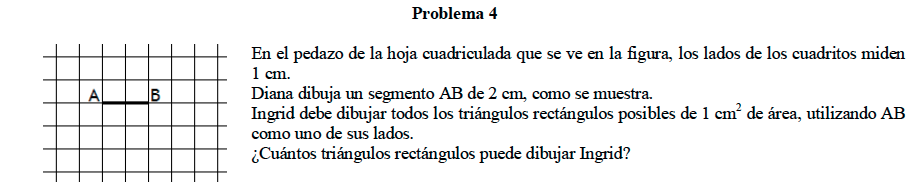
\includegraphics[width=\linewidth]{2020_05_23/imgs/OMAPA_2012_r5_B_4}
	%\caption{}
	\label{OMAPA_2012_r5_B_4}
\end{figure}

\begin{figure}[H]
	\centering
	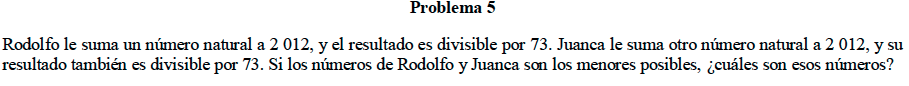
\includegraphics[width=\linewidth]{2020_05_23/imgs/OMAPA_2012_r5_B_5}
	%\caption{}
	\label{OMAPA_2012_r5_B_5}
\end{figure}

%------------------------------------------------------------------------------------------------------------   
%----------------------------------                        MEDIO                       ---------------------------------- 
%------------------------------------------------------------------------------------------------------------ 
\newpage
\section{Nivel Medio}\label{MEDIO_2020_23_mayo}

\begin{center}
	\fbox{\fbox{\parbox{6in}{\centering
				\textbf{Tiempo mínimo: } 2 horas y 30 minutos.\\
				\textbf{Tiempo máximo: } 4 horas.\\				
				\textbf{Procedimientos: }Cada problema debe estar resuelto por escrito, en forma detallada, todos los pasos seguidos para su resolución deben estar bien explicados. Se le brindarán unas hojas grapadas, en la \textit{parte de enfrente} de cada hoja debe estar la solución de los problemas, la \textit{parte posterior} no se leerá pero las operaciones y cálculos deben hacerlos allí. \\
				\textbf{Puntaje: }Cada problema vale 50 puntos, son 5, para un total de 250 puntos.
	}}}
\end{center}


\begin{figure}[H]
	\centering
	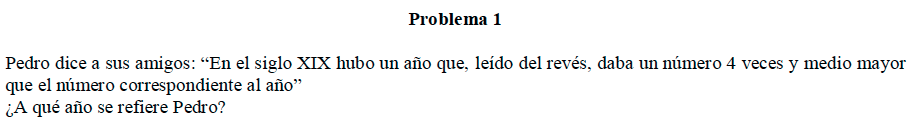
\includegraphics[width=\linewidth]{2020_05_23/imgs/OMAPA_2012_r5_M_1}
	%\caption{}
	\label{OMAPA_2012_r5_M_1}
\end{figure}

\begin{figure}[H]
	\centering
	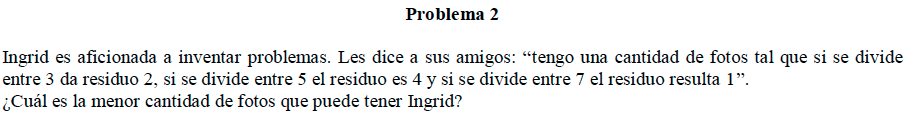
\includegraphics[width=\linewidth]{2020_05_23/imgs/OMAPA_2012_r5_M_2}
	%\caption{}
	\label{OMAPA_2012_r5_M_2}
\end{figure}

\begin{figure}[H]
	\centering
	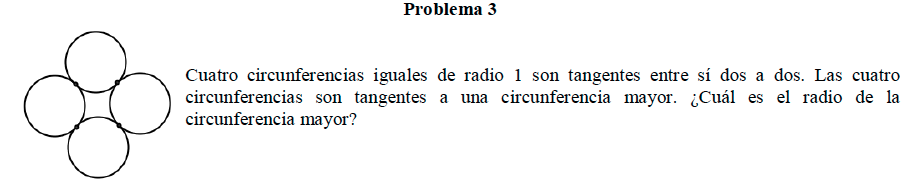
\includegraphics[width=\linewidth]{2020_05_23/imgs/OMAPA_2012_r5_M_3}
	%\caption{}
	\label{OMAPA_2012_r5_M_3}
\end{figure}

\begin{figure}[H]
	\centering
	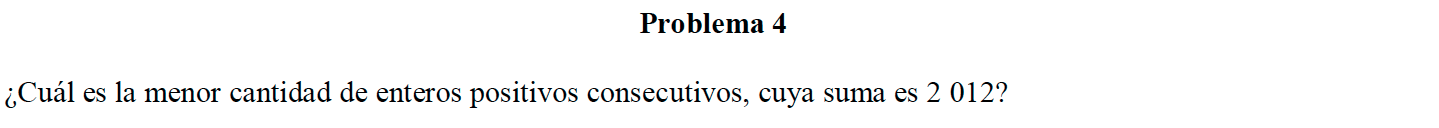
\includegraphics[width=\linewidth]{2020_05_23/imgs/OMAPA_2012_r5_M_4}
	%\caption{}
	\label{OMAPA_2012_r5_M_4}
\end{figure}

\begin{figure}[H]
	\centering
	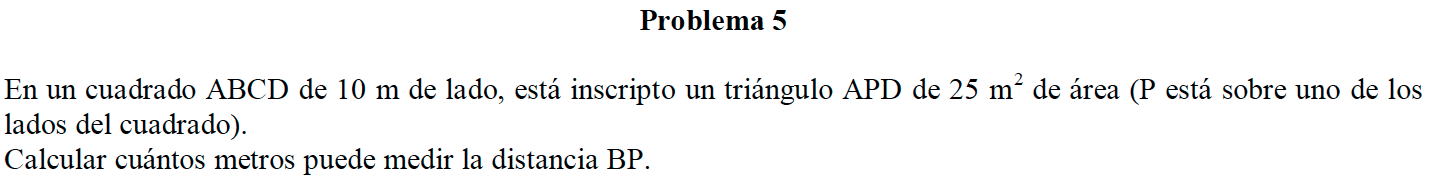
\includegraphics[width=\linewidth]{2020_05_23/imgs/OMAPA_2012_r5_M_5}
	%\caption{}
	\label{OMAPA_2012_r5_M_5}
\end{figure}

%------------------------------------------------------------------------------------------------------------   
%----------------------------------                        AVANZADO                       ---------------------------------- 
%------------------------------------------------------------------------------------------------------------ 

\newpage
\section{Nivel Avanzado}\label{AVANZADO_2020_23_mayo}

\begin{center}
	\fbox{\fbox{\parbox{6in}{\centering
				\textbf{Tiempo mínimo: } 2 horas y 30 minutos.\\
				\textbf{Tiempo máximo: } 4 horas.\\		
				\textbf{Procedimientos: }Cada problema debe estar resuelto por escrito, en forma detallada, todos los pasos seguidos para su resolución deben estar bien explicados. Se le brindarán unas hojas grapadas, en la \textit{parte de enfrente} de cada hoja debe estar la solución de los problemas, la \textit{parte posterior} no se leerá pero las operaciones y cálculos deben hacerlos allí. \\
				\textbf{Puntaje: }Cada problema vale 50 puntos, son 5, para un total de 250 puntos.
	}}}
\end{center}


\begin{figure}[H]
	\centering
	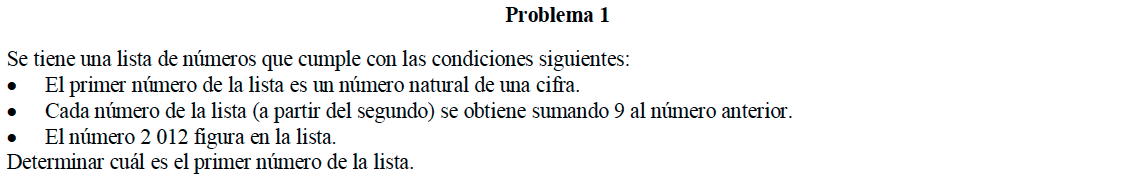
\includegraphics[width=\linewidth]{2020_05_23/imgs/OMAPA_2012_r5_A_1}
	%\caption{}
	\label{OMAPA_2012_r5_A_1}
\end{figure}

\begin{figure}[H]
	\centering
	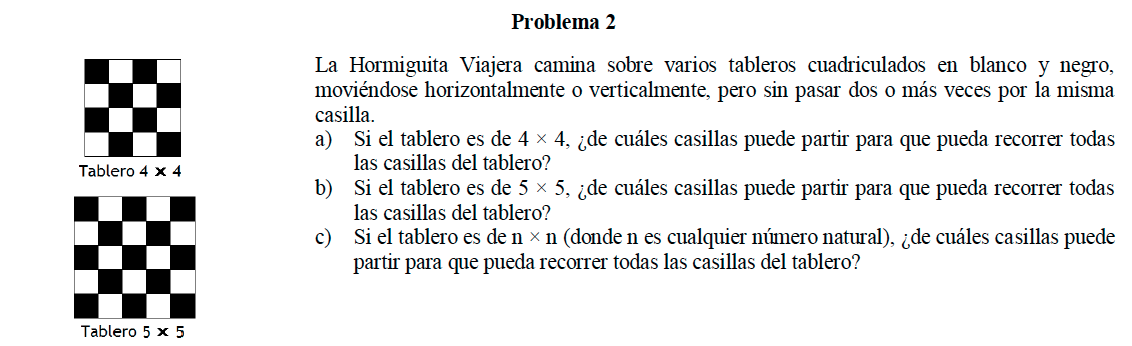
\includegraphics[width=\linewidth]{2020_05_23/imgs/OMAPA_2012_r5_A_2}
	%\caption{}
	\label{OMAPA_2012_r5_A_2}
\end{figure}

\begin{figure}[H]
	\centering
	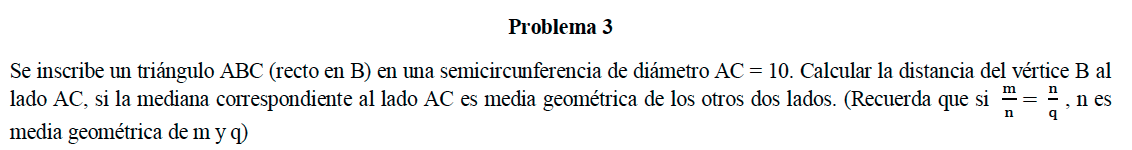
\includegraphics[width=\linewidth]{2020_05_23/imgs/OMAPA_2012_r5_A_3}
	%\caption{}
	\label{OMAPA_2012_r5_A_3}
\end{figure}

\begin{figure}[H]
	\centering
	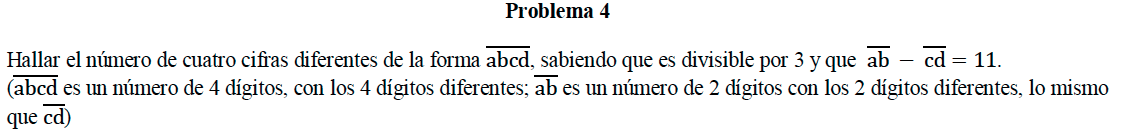
\includegraphics[width=\linewidth]{2020_05_23/imgs/OMAPA_2012_r5_A_4}
	%\caption{}
	\label{OMAPA_2012_r5_A_4}
\end{figure}

\begin{figure}[H]
	\centering
	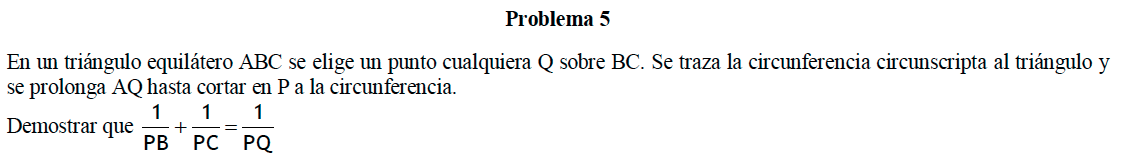
\includegraphics[width=\linewidth]{2020_05_23/imgs/OMAPA_2012_r5_A_5}
	%\caption{}
	\label{OMAPA_2012_r5_A_5}
\end{figure}